% !TEX program = pdflatex
\documentclass[review,12pt,authoryear]{elsarticle}
\usepackage{amsmath,amssymb}
\usepackage{array}
\usepackage{booktabs}
\usepackage[tableposition=top]{caption}
\usepackage{enumitem}
\usepackage{tikz}
\usepackage{pgfplots}
\pgfplotsset{compat=1.18}
\usepackage{url}
\urlstyle{same}
\def\UrlBreaks{\do\-\do\_\do\/}
\def\UrlBigBreaks{}
\usepackage{adjustbox}
\usepackage{graphicx}
\usepackage{lineno}
\usepackage[hidelinks]{hyperref}
\emergencystretch=3em
% first-page footer: the page number alone
\makeatletter
\def\ps@pprintTitle{\let\@oddhead\@empty\let\@evenhead\@empty
  \def\@oddfoot{\hfil\thepage\hfil}\let\@evenfoot\@oddfoot}
\makeatother

% ---- notation ---------------------------------------------------------------
\newcommand{\um}{\,$\mu$m}
\newcommand{\kms}{km\,s$^{-1}$}
\newcommand{\flux}{erg\,cm$^{-2}$\,s$^{-1}$}
\newcommand{\mA}{m\AA}
\newcommand{\sci}[2]{#1\times10^{#2}}
\newcommand{\ion}[2]{#1\,\textsc{#2}}
\newcommand{\nuc}[2]{$^{#1}$#2}
\newcommand{\lxl}{$L_X/L_\mathrm{bol}$}

\begin{document}

\begin{frontmatter}

\title{(883607) 2016 TA56: A candidate dark comet on a Jupiter-family orbit}

\author{Charles C. Norton}

\begin{abstract}
Dark comets are near-Earth objects whose orbits require non-gravitational accelerations
of cometary magnitude although no coma is detected. We compare the $611$ transverse
non-gravitational terms that JPL has fitted to asteroid orbits with the largest
acceleration absorbed sunlight can produce and with DAMIT spin poles. All $14$ drifts with
known poles have the sign expected from the spin. Five accelerations exceed this
radiation limit at $500$\,kg\,m$^{-3}$ and albedo $0.5$: four belong to published dark
comets or an active asteroid, and the fifth to (883607) 2016 TA56, on a Jupiter-family
orbit ($T_J=2.69$) and not previously listed among dark comets. A fit of its $102$
positions gives $A_2=(-3.45\pm0.37)\times10^{-12}$\,au\,d$^{-2}$, $9\sigma$ weighting each
night as one position and $13\sigma$ under a night-level covariance fitted to the
residuals, if a 2007 precovery is the same object; without that night,
$A_2=(-2.2\pm4.3)\times10^{-12}$\,au\,d$^{-2}$. The 2007 images support the
identification: among all positions that orbits fitted to the later apparitions allow,
the precovery source is the only one, nothing lies at the gravity-only position to
$3.9$\,mag below it, and no other moving source shares its motion. NEOWISE gives a
diameter of $1.4$ to $3.7$\,km and an albedo of $0.050$ to $0.007$, at which the
acceleration is $15$ to $39$ times the radiation limit at $1000$\,kg\,m$^{-3}$. A single
position in 2030 would measure $A_2$ to $\pm0.4\times10^{-12}$\,au\,d$^{-2}$ independently of
the precovery. The screen recovers, retrospectively, the weakly active comet (875163)
1998 SH2 (Farnocchia et al., 2026), whose acceleration relative to the radiation limit is
a twentieth of that of 2016 TA56.
\end{abstract}

\begin{keyword}
Comets \sep Near-Earth objects \sep Asteroids \sep Celestial mechanics \sep Orbit determination
\end{keyword}

\end{frontmatter}

\linenumbers

% =============================================================================
\section{Introduction}\label{sec:intro}
% =============================================================================

Astrometry can reveal departures from a purely gravitational orbit. The thermal
re-emission of absorbed sunlight, delayed by the body's rotation, produces the Yarkovsky
drift, which JPL's orbit solutions model as a transverse acceleration $A_2$ scaling as
$r^{-2}$ \citep{Farnocchia2013}, and outgassing from an active comet produces larger
accelerations \citep{Marsden1973}. Some near-Earth objects show accelerations too large for
radiation forces but no detectable coma. These dark comets \citep{Seligman2023} divide into
an inner population of small bodies on near-circular orbits and an outer population of
larger bodies on eccentric, Jupiter-family-like orbits \citep{Seligman2024}, and their
accelerations imply outgassing at rates too low for the associated dust to be detected;
\citet{Seligman2024} list fourteen such objects. \citet{Farnocchia2026} found
that the 1998--2025 astrometry of the near-Earth object (875163) 1998 SH2 shows
perturbations consistent with outgassing, detected a weak tail of low surface brightness
during its 2025 close approach that archival images had not revealed, and proposed that
non-gravitational perturbations over long astrometric arcs can identify further comets
among near-Earth objects classified as asteroids.

We present such a search: a screen of every transverse term in the JPL Small-Body
Database for accelerations larger than absorbed sunlight can produce (the radiation
limit), and for drifts of the wrong sign for the body's known spin. Of the thirteen
published dark comets with a transverse term, the screen recovers the six whose terms
exceed the radiation limit, and it identifies one further object, 2016 TA56; under typical
assumptions for density and albedo it also flags 1998 SH2, recovering retrospectively a
weakly active comet from its non-gravitational acceleration alone. Such a search was
proposed by \citet{Farnocchia2026}; this work contributes the screen and
the candidate it identifies.

Section~\ref{sec:method} describes the data and methods. Section~\ref{sec:results} presents
the screen, an independent orbit determination for 2016 TA56, the tests of its 2007
precovery in the archival images, its size and albedo from NEOWISE, the minimum outgassing
rate, the 2030 apparition, an overview of the tests, and the same analysis of the two
further objects that the screen identifies, 1998 SH2 and 2006 VC.
Section~\ref{sec:related} relates the results to previous work, and
Section~\ref{sec:conclusion} summarises the conclusions.

% =============================================================================
\section{Data and methods}\label{sec:method}
% =============================================================================

\emph{The screen.} The Small-Body Database query API returns every asteroid with a
transverse term $A_2$ (au\,d$^{-2}$ at $1$\,au) and its uncertainty, with $H$, any
measured diameter and the orbital elements; we queried it on 2026 October 16 for every
asteroid whose orbit solution includes $A_2$, and the query and its raw result are
available in the repository given under Data availability. Each term is compared with an
upper bound on the transverse acceleration that sunlight can impart. A sphere of
diameter $D$ at $1$\,au intercepts the power $S\pi D^2/4$, with $S=1361$\,W\,m$^{-2}$.
Absorbed photons arrive from the Sun and exert a purely radial force, so a transverse force
can come only from light that leaves the body, reflected or re-emitted; its momentum flux
is at most the intercepted power divided by $c$, a value reached only if all of it leaves
in one direction along the orbit. Dividing by the mass $\rho\pi D^3/6$ of a body of
uniform bulk density $\rho$ gives
\begin{equation}
a_{\max}=\frac{S\pi D^2/4}{c\,\rho\pi D^3/6}=\frac{3}{2}\,\frac{S/c}{\rho D},
\label{eq:amax}
\end{equation}
which we call the radiation limit, with $S/c=4.54\times10^{-6}$\,N\,m$^{-2}$. An
efficiency $\xi=|A_2|/a_{\max}$ greater than one therefore requires a force other than
radiation. The limit is a ceiling: thermal recoil re-emits most of the absorbed energy in
directions that cancel, and a ratio below one does not show that radiation can supply an
acceleration. We evaluate $\xi$ at the smallest diameter allowed by $H$ (albedo $0.5$,
unless a diameter has been measured) with $\rho=500$\,kg\,m$^{-3}$, and again at
$2000$\,kg\,m$^{-3}$ and albedo $0.14$. The diurnal component of thermal recoil drives a
prograde rotator outward and a retrograde rotator inward, while the seasonal component,
largest at $90^\circ$ obliquity, drives any rotator inward \citep{Vokrouhlicky2015}. A
retrograde rotator therefore cannot drift outward whatever its thermal properties, whereas
a prograde rotator near $90^\circ$ obliquity can drift inward. Each drift significant at
$3\sigma$ is compared with the obliquity of every pole solution in
DAMIT \citep{Durech2010}, with the orbit normal from the osculating inclination and node.

\emph{Astrometry.} The Minor Planet Center lists $102$ optical positions of 2016 TA56,
from a precovery on 2007 September 14 to 2026 June 10, in six apparitions: $12$
positions on one night in 2007, $79$ from its discovery by Pan-STARRS on 2016 October 10
to 2017 June, and $2$, $4$, $3$ and $2$ in 2020 November, 2022 August, 2025 October and
2026 June. Twenty-three of them are NEOWISE positions from twenty exposures, each with the
spacecraft's geocentric position on the second line of the record.

\emph{Orbit fits.} We integrate orbits with ASSIST \citep{Holman2023}, which is built on
REBOUND \citep{Rein2012} and its IAS15 integrator \citep{Rein2015}, using the DE440
planetary ephemeris \citep{Park2021}, the sixteen most massive asteroids, the oblateness of
the Sun and the Earth, and general relativity. The transverse acceleration is
$A_2\,g(r)$ with $g(r)=r^{-2}$, as in JPL's solution. A ground site's position is computed
from its MPC parallax constants and transformed into the GCRS with
astropy \citep{Astropy2022}; a NEOWISE position uses the reported spacecraft position. Each
model position is corrected for light time but not for aberration, which affects the
reference stars of the reduction equally. The fit adjusts the barycentric state at TDB
$2457746.5$ (2016 December 24) and, where included, $A_2$, by Gauss--Newton iteration
with forward-difference partial derivatives. Each site is weighted by its rms residual
over its retained positions where it has five or more, with a floor of $0.15''$, and by
$0.5''$ otherwise; a position whose two-coordinate $\chi^2$ exceeds $8$ is excluded at
each iteration and readmitted if it falls below that value. Positions from the same night
share the reference catalogue, the observer's clock and the seeing, so their errors are
correlated, and we therefore repeat each fit under two further weightings: that of
\citet{Veres2017}, used in JPL's solutions, which inflates the
uncertainties of more than four positions from one station on one night by $\sqrt{N/4}$,
and one that inflates every position of a night by $\sqrt{N}$ across all stations, so
that each night carries the weight of a single position. We fit gravity only, $A_2$, the
radial term $A_1$ together with $A_2$, and $A_2$ with each apparition omitted in turn, and
compare each apparition with the gravity-only orbit fitted to the others, decomposing its
residuals along and across the apparent motion. We also estimate the correlation within a
night from the residuals, with a covariance in which each position's site variance is
scaled by $s^2$ and any two positions of one night share a variance $\tau^2$ in each
coordinate, $s$ and $\tau$ set by restricted maximum likelihood. For the precovery night,
the positions that the other apparitions allow are those of the orbit fitted without that
night with $A_2$ held at each value from $-16$ to $+12\times10^{-12}$\,au\,d$^{-2}$, the
state at its conditional mean given $A_2$ under that fit's covariance; with $A_1$ also free,
the covariance of the predicted position shows how far a radial term can move it.

\emph{Precovery images.} We remeasured all sixteen CFHT MegaCam exposures of the
precovery night (300 and 420\,s), independently of the published reports. Each CCD is registered to Gaia DR3 stars
with proper motions propagated to 2007, by a quadratic map from detector pixels to the
pixels of the archive's world coordinate system. Cosmic rays are replaced by the median of
their neighbourhood, and sources are found in each CCD with a Gaussian filter for point
sources and with a filter trailed by the object's motion during the exposure. A source above
$5\sigma$ is classed as static when three other frames contain a source above $3\sigma$
within $1.2''$ of it; the remaining sources are linked into straight tracks that require
detections in six or more frames within $0.6''$ of the track, an rms residual of at most
$0.3''$, and a source within $0.6''$ of the track in at least 60 per cent of the frames
whose CCDs cover it. Repeating the linking with the frame times permuted, which destroys
real tracks, gives the rate of spurious tracks, and synthetic copies of the object,
trailed and scaled to its flux in each band, injected along $300$ random tracks
within $10''$ per hour and $20^\circ$ of its motion and from $0.5$\,mag brighter to
$2$\,mag fainter, give the completeness. To test each position at which an orbit could place the object, we sample the
trailed filter's S/N there in every frame, divide it by the median S/N of the detection in
that band, and take the median over the frames: the result is the flux, in units of the
detection's, of any source moving with the object through that position, and a static
source that crosses one or two frames does not change it. A frame's measurement is left
out within $4''+3''(18-G)$ of a Gaia star brighter than $G=18$, within $2.5''$ of a static
source above S/N $20$, and within $10''$ of the edge of its CCD, and a position requires
measurements in at least eight frames.

\emph{Thermal fit.} For each NEOWISE position the single-exposure source table gives the
W1 ($3.4\,\mu$m) and W2 ($4.6\,\mu$m) profile-fit magnitudes \citep{Wright2010,Mainzer2014},
and Horizons gives the distances from the Sun and from WISE and the phase angle. We fit
the fluxes for the diameter $D$ and the beaming parameter $\eta$ with the near-Earth
asteroid thermal model \citep{Harris1998}, with emissivity $0.9$ and no night-side
emission, plus reflected sunlight from the $H$--$G$ phase law \citep{Bowell1989}
($G=0.15$), a $5778$\,K solar spectrum and an infrared albedo $1.6$ times the
visible \citep{Mainzer2011}; the visible albedo follows from $H$. Each flux carries its
photometric uncertainty plus a $10$ per cent floor for the colour corrections and the
calibration.

% =============================================================================
\section{Results}\label{sec:results}
% =============================================================================

\subsection{The screen}

Of the $611$ asteroids with a transverse term in the database on 2026 October 16, $567$
have it at $3\sigma$ or more, and $14$ of these have DAMIT pole solutions; Table~S1 of
the supplementary material lists all $611$ with their terms, diameters, efficiencies,
pole solutions and spin-sign checks. All $14$ drifts have the sign expected from the
spin: no retrograde rotator drifts outward and no prograde rotator inward, and for the
four objects with two pole solutions both solutions give the same sense of rotation. The
eleven retrograde rotators, with obliquities of $118$ to $179^\circ$, all drift inward,
which tests the signs of their terms directly; the three prograde rotators, at $10$ to
$48^\circ$, all drift outward, and only (1580) Betulia, at $118^\circ$, lies within
$30^\circ$ of $90^\circ$. Under the typical assumptions the $567$ significant terms have a
median efficiency of $0.075$, and $95$ per cent of them lie below $0.17$. Five
accelerations exceed the radiation limit at $500$\,kg\,m$^{-3}$ and albedo $0.5$
(Table~\ref{tab:screen}): those of the active asteroid 362P/(2008 GO98), of the dark
comets 2012 UR158, 2005 UY6 and (523599) 2003 RM \citep{Seligman2023,Seligman2024}, and of
2016 TA56. At $2000$\,kg\,m$^{-3}$ and albedo $0.14$, ten exceed it, including the dark
comets 1998 FR11, 2001 ME1 and 2006 RH120 and two objects absent from the dark-comet
lists, 1998 SH2 and 2006 VC, with efficiencies of $1.6$ and $1.3$; Section~\ref{sec:others}
analyses both, and 1998 SH2 is a comet \citep{Farnocchia2026}. Only 2016 TA56 exceeds the
limit under the conservative assumptions without appearing in a published list of dark comets
or active asteroids. Thirteen of
the fourteen published dark comets have a transverse term in the database, and the
screen flags six of them. The other seven are the inner dark comets of $4$ to $21$\,m,
whose transverse terms are $0.01$ to $0.09$ of the radiation limit for bodies of their
size and whose published accelerations are based on the radial and normal terms (five of
the seven have $A_3$ at $3.6$ to $10.7\sigma$) and on thermal models of the bodies, which
a transverse screen cannot test. The screen is therefore sensitive to large dark comets
of the outer population, while the inner population is identified through the radial
terms. The screen evaluates terms that JPL has already fitted, and JPL fits $A_2$ only
where the astrometry requires or can constrain it: the $611$ include $609$ of the
$42{,}772$ near-Earth asteroids in the database, and two other objects. It finds dark
comets only among bodies whose transverse accelerations are already measured, it says
nothing about the other near-Earth objects, and the number it finds is not an estimate of
how common dark comets are.

\begin{table}[t]
\centering\small
\caption{Transverse accelerations above the radiation limit at $500$\,kg\,m$^{-3}$ and
albedo $0.5$ (or at a measured diameter). $D_{\min}$ is the diameter used, $\xi$ the ratio
of the acceleration to $a_{\max}$ at that diameter, and $\xi_{\rm typ}$ the same ratio at
$2000$\,kg\,m$^{-3}$ and albedo $0.14$.}
\label{tab:screen}
\begin{adjustbox}{max width=\textwidth}
\begin{tabular}{lrrrrrl}
\toprule
Object & $A_2$ ($10^{-12}$\,au\,d$^{-2}$) & S/N & $D_{\min}$ (m) & $\xi$ & $\xi_{\rm typ}$ & $T_J$, status \\
\midrule
362P/(2008 GO98) & $-1150$ & $11.2$ & $4921$ & $8333$ & $62990$ & 2.93, active \\
2012 UR158 & $-7.20$ & $119$ & $629$ & $6.67$ & $26.7$ & 3.00, dark comet \\
(883607) 2016 TA56 & $-3.19$ & $8.9$ & $445$ & $2.08$ & $15.8$ & 2.69, this work \\
(452639) 2005 UY6 & $-0.54$ & $11.3$ & $2249$ & $1.78$ & $7.12$ & 2.94, dark comet \\
(523599) 2003 RM & $+3.29$ & $110$ & $223$ & $1.08$ & $8.15$ & 2.95, dark comet \\
\bottomrule
\end{tabular}
\end{adjustbox}
\end{table}

\subsection{The orbit of 2016 TA56}

JPL's solution 23 (2026 June 17) uses $94$ of the positions and gives
$A_2=(-3.19\pm0.36)\times10^{-12}$\,au\,d$^{-2}$, an $8.9\sigma$ detection, with
$a=2.69$\,au, $e=0.782$, $q=0.588$\,au, aphelion $4.80$\,au, $i=32.3^\circ$, a minimum
orbit intersection distance with Jupiter of $0.185$\,au and the most recent perihelion on
2026 January 13. Our fits (Table~\ref{tab:fits}) reproduce the term. With site weights,
the fit with $A_2$ retains $97$ of the $102$ positions at an rms of $0.33''$ and gives
$A_2=(-3.54\pm0.17)\times10^{-12}$\,au\,d$^{-2}$; this uncertainty treats the twelve
precovery positions as independent. With the same-night deweighting used in JPL's fits,
which inflates the eight positions from site T14 by $\sqrt{2}$, the result is
$(-3.56\pm0.19)\times10^{-12}$; with the whole night weighted as a single position, the
limit in which the two reports share all their errors, it is
$(-3.45\pm0.37)\times10^{-12}$, a $9\sigma$ detection consistent with JPL's uncertainty.
The value is the same under all three weightings, and we adopt the last. The deweighted
fits have $\chi^2$/dof well below one because inflating the uncertainties of a night's
positions gives them the weight of one, so their $\chi^2$ reflects the weighting rather
than the size of the errors, and the site-weighted fit's $0.65$ reflects the $0.15''$
floor on sites whose scatter is smaller. A fourth treatment estimates the correlation from
the residuals: each position's site variance is scaled by $s^2$, and any two positions of
the same night share a variance $\tau^2$ in each coordinate. Restricted maximum likelihood
over the $97$ positions kept on $28$ nights gives $s=0.68$ and $\tau=0.17''$ ($95$ per cent
interval $0.11$ to $0.23''$), and with this covariance
$A_2=(-3.85\pm0.30)\times10^{-12}$, a $13\sigma$ term, or
$(-3.88\pm0.37)\times10^{-12}$ with $\tau$ at its upper bound. Weighting each night as one
position is therefore the more conservative treatment. These uncertainties belong to fits
that include the 2007 night; the dependence on that night, and the possibility that its
source is a different object, are examined in Section~\ref{sec:precovery}. Omitting one night at a time, the
one-position-per-night fit gives $A_2$ between $-3.96$ and $-3.39\times10^{-12}$ for every
night after 2007, a jackknife uncertainty of $0.53\times10^{-12}$ that corresponds to
$6.5\sigma$; resampling those nights with replacement, with the 2007 night always included,
gives a $95$ per cent interval of $-4.9$ to $-3.2\times10^{-12}$ over $200$ samples.
Clipping thresholds of $6$, $12$ and none, error floors of $0.10$ and $0.25''$, and
default uncertainties of $0.3$ and $0.8''$ change the term by at most
$0.14\times10^{-12}$, with significances between $7.4$ and $10.6\sigma$. A radial term
fitted simultaneously is $A_1=(+3.7\pm1.9)\times10^{-10}$\,au\,d$^{-2}$, $2\sigma$ from
zero, with $A_2=(-3.32\pm0.21)\times10^{-12}$: the radial term, which the geometry of a
single precovery night constrains poorly, does not absorb the transverse one. The
gravity-only fit retains $83$ positions, rejecting all twelve from 2007 and all three
from 2025 October.

\begin{table}[t]
\centering\small
\caption{Orbit fits of 2016 TA56 to the $102$ MPC positions. The first three fits differ
in the weighting of positions from the same night (Section~\ref{sec:method}).}
\label{tab:fits}
\begin{adjustbox}{max width=\textwidth}
\begin{tabular}{lrrrl}
\toprule
Fit & Positions & Kept & $\chi^2$/dof & $A_2$ ($10^{-12}$\,au\,d$^{-2}$) \\
\midrule
with $A_2$, site weights & 102 & 97 & 121.2/187 & $-3.54\pm0.17$ \\
with $A_2$, nights deweighted by $\sqrt{N/4}$ & 102 & 97 & 105.8/187 & $-3.56\pm0.19$ \\
with $A_2$, one position a night & 102 & 101 & 58.2/195 & $-3.45\pm0.37$ \\
with $A_1$ and $A_2$ & 102 & 97 & 117.3/186 & $-3.32\pm0.21$, $A_1=+367\pm187$ \\
gravity only & 102 & 83 & 112.8/160 & --- \\
without 2007 September & 90 & 85 & 118.2/163 & $-2.24\pm4.34$ \\
without 2016--2017 & 23 & 21 & 2.5/35 & $-4.80\pm3.20$ \\
without 2020 November & 100 & 95 & 120.4/183 & $-3.55\pm0.17$ \\
without 2022 August & 98 & 93 & 120.8/179 & $-3.54\pm0.18$ \\
without 2025 October & 99 & 95 & 116.1/183 & $-3.79\pm0.57$ \\
without 2026 June & 100 & 95 & 120.8/183 & $-3.54\pm0.17$ \\
\bottomrule
\end{tabular}
\end{adjustbox}
\end{table}

\subsection{Dependence on the 2007 precovery}\label{sec:precovery}

Omitting the 2007 precovery gives $A_2=(-2.2\pm4.3)\times10^{-12}$\,au\,d$^{-2}$, of the
same sign but no longer significant; omitting any other apparition except the discovery
apparition leaves it above $6\sigma$. Resampling all $28$ nights with replacement gives a
term beyond $3\sigma$ in $57$ per cent of $200$ samples, close to the $64$ per cent of
samples that include the 2007 night, so nearly every significant resample contains it.
The detection is therefore conditional on the precovery: with that night the term is
measured at $9$ to $13\sigma$, according to the treatment of same-night errors, and
without it the later apparitions do not measure it. Under the night-level covariance, the
twelve 2007 positions would have to share a further error of $0.68''$ in each coordinate
to bring $A_2$ down to $5\sigma$, and of $1.20''$ to bring it to $3\sigma$. The twelve precovery positions come from two reports
from Mauna Kea (sites 568 and T14) for 2007 September 14, with four and eight positions
interleaved over $78$ minutes and consecutive frames of each report at least $7.0$ (568)
and $5.8$ minutes (T14) apart, in the D1 field of the CFHT Legacy Survey, where the
predicted motion was $34.5''$ per hour toward position angle $210^\circ$. Both reports are
re-measurements of the same CFHT frames against Gaia DR2, so they share the frame timing
and the reference catalogue: they are two reductions of one night, not two independent
nights. The gravity-only orbit fitted to the later apparitions predicts the positions for
that night with uncertainties of $0.08''$ along the apparent motion and $0.20''$ across
it, from its covariance; the precovery positions lie $3.45''$ from that prediction,
$1.8''$ along the motion and $3.0''$ across it, with a scatter of $0.07''$
(Figure~\ref{fig:oc}a).

A timing error displaces a position only along the apparent motion. It could therefore
account for the along-track offset, which corresponds to three minutes, but not for the
cross-track offset, which is fifteen times the prediction uncertainty whether or not the
two reports share a clock. Both reports use Gaia DR2 as the reference catalogue, which
rules out a catalogue offset of this size. We measured the CFHT frames independently
(Table~\ref{tab:cfht}, Figure~\ref{fig:cutouts}), registering each to Gaia DR3 stars with
proper motions propagated to 2007, with a median rms of $0.02''$. The object is detected
in twelve frames, each time trailed by its motion during the exposure ($4.06''$ in the
$420$\,s $r$ frames and $2.90''$ in the $300$\,s $g$ frames), along a straight track
from which both reports deviate by $0.10''$ rms across the motion. In eleven frames our
centroid lies within $0.42''$ of the accelerated orbit and $3.2$ to $3.4''$ east of the
gravity-only orbit; in frame 942303, where the object is faint, it lies $1.7''$ away, and
in frame 942308, where the object is next to a star, it is not detected. The offset is
therefore present in the images rather than introduced by either reduction, and removing
the transverse term would require a common error of $3.0''$ across the motion in every
position, $150$ times the scatter of the registration. With $A_2$ the precovery positions
are fitted to within $0.07''$ (Figure~\ref{fig:oc}c).

The later positions support the same conclusion. A gravity-only orbit fitted to the
precovery and the apparitions through 2022 fits the precovery but misses the three
positions of 2025 October by $10.5''$ ($6.7''$ along and $8.0''$ across the motion),
against a prediction uncertainty of $0.4''$, and the two of 2026 June by $2.3''$, which
the fit then rejects (Figure~\ref{fig:oc}b). No gravity-only orbit fits the precovery and
the last two apparitions together, while the orbit with the transverse term fits all of
them. The term is therefore robust unless the precovery is a different object. A
misidentification would leave a body whose 2016--2026 arc constrains $A_2$ only to
$\pm4.3\times10^{-12}$\,au\,d$^{-2}$, and strong non-gravitational accelerations can
themselves complicate the linking of observations \citep{Taylor2024b}. The three
reductions of that night agree to $0.2''$, and the measured motion, $34.7''$ per hour
toward position angle $209^\circ$, is the rate and direction predicted by the orbit.

The 2007 frames test the identification directly, because 2016 TA56 must appear in them
whatever its acceleration. Every orbit fitted to the later apparitions places it on one
line through the gravity-only position, $0.93''$ further west for each $10^{-12}$\,au\,d$^{-2}$
of $A_2$, and a radial term fitted as well moves it only along the same line ($1\sigma$
ellipse $4.05''\times0.17''$). Its absolute magnitude predicts $V=23.1$ that night, and the
measured source has $r=22.8$.
Along this line the frames show a single source (Figure~\ref{fig:locus}): the median flux
reaches $0.96$ of the detection's at $A_2=-3.75\times10^{-12}$\,au\,d$^{-2}$ and is nowhere
else above $0.05$, and within $24''$ of the gravity-only position in any direction
nothing but the detection exceeds $0.13$. At the
gravity-only position it is $-0.04$, while lines displaced across the field give a robust
scatter of $0.022$ at the same point, so any object there is at least $3.9$\,mag
fainter than the detection ($3\sigma$). Of the $954$ displaced lines, none reach half the
detection's flux anywhere along their length. The precovery source is therefore
2016 TA56 unless that object was about $40$ times fainter than its absolute magnitude
implies while an unrelated object moving as predicted lay on the line.

A census of the moving sources in all sixteen frames measures the density of such objects
in these images, rather than among known asteroids. It finds $68$ moving sources besides
2016 TA56 over the $0.86$\,deg$^2$ of the mosaic, $79$ per square degree, among them
$21$ of the $22$ known asteroids with good positions that
SkyBoT \citep{Berthier2006} places on the frames. They move at $22\pm13''$ per hour; none
comes within $5''$ per hour and $10^\circ$ of the object's motion, and three within
$10''$ per hour and $20^\circ$. Injected copies of the object are recovered on $109$ of
the $115$ tracks placed within $0.5$\,mag of its brightness, and no track forms with
the frame times shuffled. With normal distributions fitted to the rates and directions of
the census, the expected number of unrelated objects within $30''$ of the predicted
position and within $0.5''$ per hour and $1^\circ$ of the measured motion is $8\times10^{-6}$.

The 2007 night is the only epoch before the discovery that constrains the orbit. The
other images of the predicted track listed by the CADC SSOIS index recorded the object at
$V=23.2$ or fainter, beyond the depth of their exposures: forced photometry at the
predicted position gives S/N $0.9$ and $2.2$ in the deepest, two DECam exposures of
2013 September 29 at $V=23.9$, and $1.4$ in a stack of eight Pan-STARRS1 exposures of
2013 August, and the accelerated and gravity-only orbits are only $0.5''$ apart in 2013.

\begin{figure}[tp]
\centering
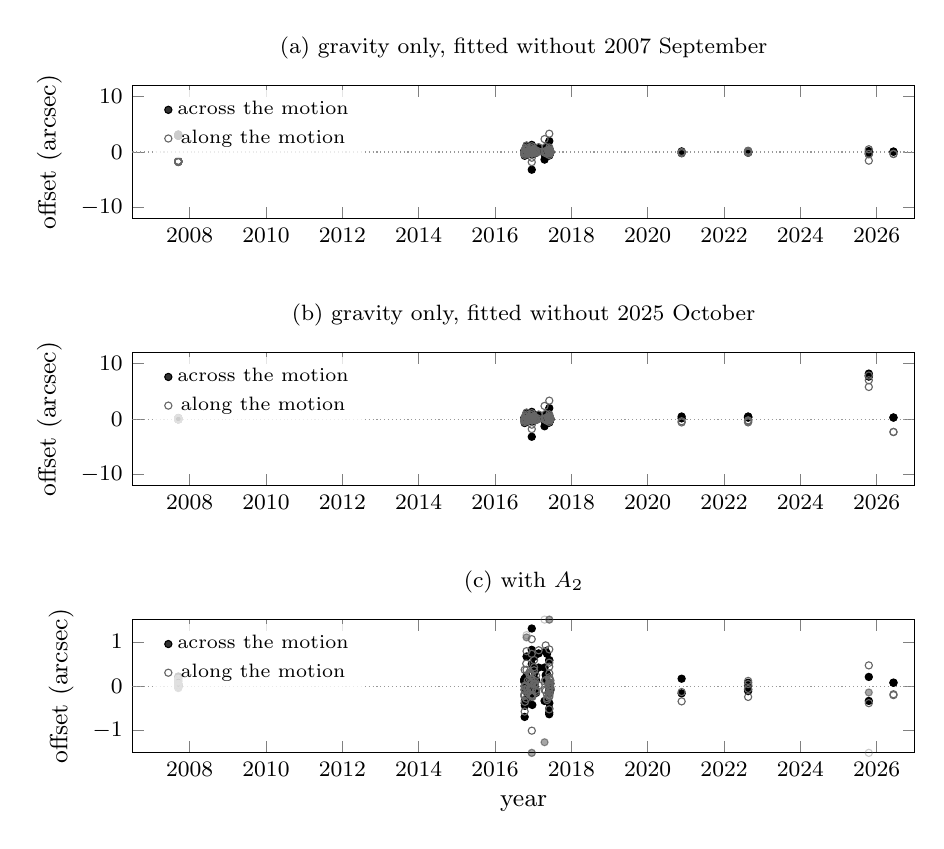
\begin{tikzpicture}
\begin{axis}[name=p0,width=0.95\textwidth,height=0.27\textwidth,xmin=2006.5,xmax=2027,ymin=-12,ymax=12,
  xlabel={},ylabel={offset (arcsec)},title={(a) gravity only, fitted without 2007 September},title style={font=\footnotesize},tick label style={font=\footnotesize},
  label style={font=\small},x tick label style={/pgf/number format/1000 sep={}},legend style={font=\scriptsize,at={(0.03,0.97)},anchor=north west,draw=none,fill=white,fill opacity=0.8,text opacity=1},legend columns=1]
\addplot[only marks,mark=*,mark size=1.3pt,black] coordinates {(2007.701,3.13) (2007.702,2.95) (2007.702,2.97) (2007.702,2.97) (2007.702,3.01) (2007.702,2.96) (2007.702,3.17) (2007.702,3.00) (2007.702,2.99) (2007.702,2.97) (2007.702,2.95) (2007.702,2.96) (2016.767,0.17) (2016.767,0.13) (2016.775,0.19) (2016.775,0.15) (2016.775,0.11) (2016.775,0.16) (2016.777,-0.35) (2016.777,0.03) (2016.777,-0.67) (2016.783,-0.41) (2016.783,-0.05) (2016.783,-0.29) (2016.818,0.02) (2016.818,0.05) (2016.826,1.13) (2016.826,0.27) (2016.826,0.70) (2016.856,-0.15) (2016.856,0.16) (2016.856,-0.25) (2016.900,-0.06) (2016.900,-0.10) (2016.900,-0.20) (2016.930,-0.14) (2016.930,0.05) (2016.930,-0.12) (2016.961,0.82) (2016.961,0.07) (2016.962,0.50) (2016.962,0.04) (2016.963,-3.18) (2016.963,1.29) (2016.963,0.01) (2016.964,-0.21) (2016.964,0.75) (2016.964,-0.12) (2016.977,0.12) (2016.977,-0.42) (2016.977,-0.10) (2016.977,-0.05) (2017.023,0.33) (2017.023,0.64) (2017.023,0.04) (2017.042,0.29) (2017.042,-0.03) (2017.042,-0.09) (2017.075,0.70) (2017.075,0.12) (2017.075,-0.16) (2017.143,0.69) (2017.143,0.37) (2017.298,0.32) (2017.298,-0.44) (2017.298,-1.36) (2017.328,0.09) (2017.328,0.19) (2017.328,0.72) (2017.363,0.08) (2017.363,0.70) (2017.363,0.23) (2017.420,-0.63) (2017.420,-0.58) (2017.421,0.60) (2017.421,-0.02) (2017.421,0.59) (2017.421,-0.50) (2017.421,-0.13) (2017.422,-0.16) (2017.422,-0.04) (2017.422,-0.08) (2017.422,1.98) (2017.423,-0.38) (2017.423,-0.02) (2017.429,0.02) (2017.429,-0.09) (2017.429,-0.11) (2017.451,0.07) (2017.451,-0.04) (2017.451,-0.08) (2020.889,0.12) (2020.889,-0.21) (2022.631,0.07) (2022.631,-0.12) (2022.631,-0.08) (2022.631,0.01) (2025.793,0.17) (2025.793,-0.38) (2025.793,-0.18) (2026.439,0.07) (2026.439,0.07)};
\addlegendentry{across the motion}
\addplot[only marks,mark=o,mark size=1.3pt,black!60] coordinates {(2007.701,-1.59) (2007.702,-1.80) (2007.702,-1.65) (2007.702,-1.76) (2007.702,-1.62) (2007.702,-1.71) (2007.702,-1.73) (2007.702,-1.76) (2007.702,-1.65) (2007.702,-1.71) (2007.702,-1.71) (2007.702,-1.79) (2016.767,-0.13) (2016.767,-0.17) (2016.775,-0.04) (2016.775,-0.02) (2016.775,0.05) (2016.775,-0.02) (2016.777,0.06) (2016.777,0.42) (2016.777,-0.52) (2016.783,0.03) (2016.783,-0.30) (2016.783,0.04) (2016.818,-0.25) (2016.818,0.55) (2016.826,1.18) (2016.826,0.82) (2016.826,0.40) (2016.856,-0.12) (2016.856,-0.03) (2016.856,0.14) (2016.900,0.30) (2016.900,0.10) (2016.900,0.27) (2016.930,-0.09) (2016.930,0.27) (2016.930,0.06) (2016.961,0.23) (2016.961,0.71) (2016.962,1.04) (2016.962,-0.22) (2016.963,-1.81) (2016.963,0.08) (2016.963,-0.25) (2016.964,-0.23) (2016.964,0.04) (2016.964,-1.02) (2016.977,-0.08) (2016.977,-0.07) (2016.977,-0.26) (2016.977,-0.21) (2017.023,0.44) (2017.023,0.37) (2017.023,0.60) (2017.042,0.08) (2017.042,0.14) (2017.042,0.07) (2017.075,0.28) (2017.075,-0.09) (2017.075,-0.04) (2017.143,0.88) (2017.143,0.09) (2017.298,-0.10) (2017.298,0.09) (2017.298,2.33) (2017.328,0.92) (2017.328,0.15) (2017.328,-0.09) (2017.363,-0.19) (2017.363,-0.31) (2017.363,-0.27) (2017.420,-0.53) (2017.420,-0.24) (2017.421,0.03) (2017.421,0.44) (2017.421,-0.06) (2017.421,0.08) (2017.421,0.19) (2017.422,0.82) (2017.422,0.53) (2017.422,-0.21) (2017.422,3.30) (2017.423,0.28) (2017.423,0.16) (2017.429,-0.18) (2017.429,-0.13) (2017.429,-0.11) (2017.451,0.06) (2017.451,-0.02) (2017.451,0.14) (2020.889,0.01) (2020.889,-0.19) (2022.631,0.24) (2022.631,-0.12) (2022.631,0.17) (2022.631,0.07) (2025.793,-0.35) (2025.793,0.50) (2025.793,-1.55) (2026.439,-0.35) (2026.439,-0.33)};
\addlegendentry{along the motion}
\addplot[black!40,densely dotted,forget plot] coordinates {(2006.5,0) (2027,0)};
\end{axis}
\begin{axis}[name=p1,at={(p0.south)},anchor=north,yshift=-1.7cm,width=0.95\textwidth,height=0.27\textwidth,xmin=2006.5,xmax=2027,ymin=-12,ymax=12,
  xlabel={},ylabel={offset (arcsec)},title={(b) gravity only, fitted without 2025 October},title style={font=\footnotesize},tick label style={font=\footnotesize},
  label style={font=\small},x tick label style={/pgf/number format/1000 sep={}},legend style={font=\scriptsize,at={(0.03,0.97)},anchor=north west,draw=none,fill=white,fill opacity=0.8,text opacity=1},legend columns=1]
\addplot[only marks,mark=*,mark size=1.3pt,black] coordinates {(2007.701,0.17) (2007.702,-0.02) (2007.702,0.01) (2007.702,0.00) (2007.702,0.05) (2007.702,-0.01) (2007.702,0.21) (2007.702,0.04) (2007.702,0.02) (2007.702,0.00) (2007.702,-0.02) (2007.702,-0.01) (2016.767,0.14) (2016.767,0.10) (2016.775,0.16) (2016.775,0.11) (2016.775,0.08) (2016.775,0.13) (2016.777,-0.39) (2016.777,-0.01) (2016.777,-0.70) (2016.783,-0.45) (2016.783,-0.08) (2016.783,-0.33) (2016.818,-0.01) (2016.818,0.02) (2016.826,1.10) (2016.826,0.24) (2016.826,0.67) (2016.856,-0.17) (2016.856,0.14) (2016.856,-0.27) (2016.900,-0.07) (2016.900,-0.11) (2016.900,-0.21) (2016.930,-0.14) (2016.930,0.05) (2016.930,-0.12) (2016.961,0.84) (2016.961,0.09) (2016.962,0.51) (2016.962,0.06) (2016.963,-3.17) (2016.963,1.31) (2016.963,0.03) (2016.964,-0.20) (2016.964,0.76) (2016.964,-0.10) (2016.977,0.14) (2016.977,-0.40) (2016.977,-0.08) (2016.977,-0.03) (2017.023,0.36) (2017.023,0.67) (2017.023,0.08) (2017.042,0.32) (2017.042,-0.00) (2017.042,-0.06) (2017.075,0.72) (2017.075,0.14) (2017.075,-0.14) (2017.143,0.74) (2017.143,0.42) (2017.298,0.41) (2017.298,-0.35) (2017.298,-1.28) (2017.328,0.15) (2017.328,0.25) (2017.328,0.79) (2017.363,0.13) (2017.363,0.74) (2017.363,0.28) (2017.420,-0.62) (2017.420,-0.58) (2017.421,0.60) (2017.421,-0.02) (2017.421,0.59) (2017.421,-0.49) (2017.421,-0.12) (2017.422,-0.16) (2017.422,-0.04) (2017.422,-0.08) (2017.422,1.99) (2017.423,-0.37) (2017.423,-0.01) (2017.429,0.02) (2017.429,-0.10) (2017.429,-0.11) (2017.451,0.06) (2017.451,-0.05) (2017.451,-0.09) (2020.889,0.47) (2020.889,0.14) (2022.631,0.47) (2022.631,0.28) (2022.631,0.31) (2022.631,0.41) (2025.793,8.20) (2025.793,7.66) (2025.793,7.86) (2026.439,0.29) (2026.439,0.29)};
\addlegendentry{across the motion}
\addplot[only marks,mark=o,mark size=1.3pt,black!60] coordinates {(2007.701,0.14) (2007.702,-0.07) (2007.702,0.09) (2007.702,-0.03) (2007.702,0.11) (2007.702,0.02) (2007.702,0.00) (2007.702,-0.03) (2007.702,0.08) (2007.702,0.02) (2007.702,0.03) (2007.702,-0.06) (2016.767,-0.15) (2016.767,-0.19) (2016.775,-0.06) (2016.775,-0.03) (2016.775,0.03) (2016.775,-0.04) (2016.777,0.04) (2016.777,0.41) (2016.777,-0.53) (2016.783,0.02) (2016.783,-0.31) (2016.783,0.02) (2016.818,-0.25) (2016.818,0.55) (2016.826,1.19) (2016.826,0.83) (2016.826,0.41) (2016.856,-0.10) (2016.856,-0.01) (2016.856,0.16) (2016.900,0.34) (2016.900,0.13) (2016.900,0.30) (2016.930,-0.05) (2016.930,0.31) (2016.930,0.09) (2016.961,0.27) (2016.961,0.74) (2016.962,1.07) (2016.962,-0.19) (2016.963,-1.78) (2016.963,0.12) (2016.963,-0.22) (2016.964,-0.20) (2016.964,0.08) (2016.964,-0.99) (2016.977,-0.05) (2016.977,-0.05) (2016.977,-0.23) (2016.977,-0.18) (2017.023,0.43) (2017.023,0.36) (2017.023,0.59) (2017.042,0.06) (2017.042,0.12) (2017.042,0.04) (2017.075,0.25) (2017.075,-0.12) (2017.075,-0.08) (2017.143,0.83) (2017.143,0.04) (2017.298,-0.06) (2017.298,0.13) (2017.298,2.38) (2017.328,0.94) (2017.328,0.17) (2017.328,-0.08) (2017.363,-0.17) (2017.363,-0.29) (2017.363,-0.25) (2017.420,-0.50) (2017.420,-0.21) (2017.421,0.06) (2017.421,0.47) (2017.421,-0.03) (2017.421,0.11) (2017.421,0.22) (2017.422,0.85) (2017.422,0.56) (2017.422,-0.18) (2017.422,3.33) (2017.423,0.31) (2017.423,0.19) (2017.429,-0.15) (2017.429,-0.10) (2017.429,-0.08) (2017.451,0.09) (2017.451,0.01) (2017.451,0.16) (2020.889,-0.38) (2020.889,-0.59) (2022.631,-0.22) (2022.631,-0.58) (2022.631,-0.29) (2022.631,-0.39) (2025.793,7.00) (2025.793,7.86) (2025.793,5.80) (2026.439,-2.32) (2026.439,-2.30)};
\addlegendentry{along the motion}
\addplot[black!40,densely dotted,forget plot] coordinates {(2006.5,0) (2027,0)};
\end{axis}
\begin{axis}[name=p2,at={(p1.south)},anchor=north,yshift=-1.7cm,width=0.95\textwidth,height=0.27\textwidth,xmin=2006.5,xmax=2027,ymin=-1.5,ymax=1.5,
  xlabel={year},ylabel={offset (arcsec)},title={(c) with $A_2$},title style={font=\footnotesize},tick label style={font=\footnotesize},
  label style={font=\small},x tick label style={/pgf/number format/1000 sep={}},legend style={font=\scriptsize,at={(0.03,0.97)},anchor=north west,draw=none,fill=white,fill opacity=0.8,text opacity=1},legend columns=1]
\addplot[only marks,mark=*,mark size=1.3pt,black] coordinates {(2007.701,0.18) (2007.702,-0.01) (2007.702,0.02) (2007.702,0.01) (2007.702,0.06) (2007.702,0.00) (2007.702,0.22) (2007.702,0.04) (2007.702,0.03) (2007.702,0.01) (2007.702,-0.01) (2007.702,0.00) (2016.767,0.15) (2016.767,0.11) (2016.775,0.17) (2016.775,0.12) (2016.775,0.09) (2016.775,0.14) (2016.777,-0.38) (2016.777,-0.00) (2016.777,-0.69) (2016.783,-0.44) (2016.783,-0.08) (2016.783,-0.32) (2016.818,-0.01) (2016.818,0.02) (2016.826,0.24) (2016.826,0.67) (2016.856,-0.18) (2016.856,0.13) (2016.856,-0.28) (2016.900,-0.08) (2016.900,-0.12) (2016.900,-0.22) (2016.930,-0.15) (2016.930,0.03) (2016.930,-0.13) (2016.961,0.82) (2016.961,0.07) (2016.962,0.50) (2016.962,0.04) (2016.963,1.30) (2016.963,0.01) (2016.964,-0.21) (2016.964,0.75) (2016.964,-0.11) (2016.977,0.13) (2016.977,-0.42) (2016.977,-0.09) (2016.977,-0.04) (2017.023,0.35) (2017.023,0.66) (2017.023,0.07) (2017.042,0.31) (2017.042,-0.01) (2017.042,-0.07) (2017.075,0.72) (2017.075,0.14) (2017.075,-0.15) (2017.143,0.74) (2017.143,0.42) (2017.298,0.42) (2017.298,-0.33) (2017.328,0.15) (2017.328,0.25) (2017.328,0.79) (2017.363,0.12) (2017.363,0.73) (2017.363,0.27) (2017.420,-0.63) (2017.420,-0.59) (2017.421,0.59) (2017.421,-0.03) (2017.421,0.58) (2017.421,-0.50) (2017.421,-0.13) (2017.422,-0.16) (2017.422,-0.04) (2017.422,-0.09) (2017.423,-0.38) (2017.423,-0.02) (2017.429,0.01) (2017.429,-0.10) (2017.429,-0.12) (2017.451,0.06) (2017.451,-0.06) (2017.451,-0.09) (2020.889,0.17) (2020.889,-0.16) (2022.631,0.08) (2022.631,-0.11) (2022.631,-0.07) (2022.631,0.02) (2025.793,0.21) (2025.793,-0.33) (2026.439,0.08) (2026.439,0.08)};
\addlegendentry{across the motion}
\addplot[only marks,mark=*,mark size=1.3pt,black,opacity=0.35,forget plot] coordinates {(2016.826,1.10) (2016.963,-1.50) (2017.298,-1.26) (2017.422,1.50) (2025.793,-0.14)};
\addplot[only marks,mark=o,mark size=1.3pt,black!60] coordinates {(2007.701,0.17) (2007.702,-0.04) (2007.702,0.11) (2007.702,-0.00) (2007.702,0.14) (2007.702,0.05) (2007.702,0.03) (2007.702,-0.00) (2007.702,0.11) (2007.702,0.05) (2007.702,0.05) (2007.702,-0.03) (2016.767,-0.18) (2016.767,-0.22) (2016.775,-0.09) (2016.775,-0.07) (2016.775,-0.00) (2016.775,-0.07) (2016.777,0.01) (2016.777,0.37) (2016.777,-0.57) (2016.783,-0.01) (2016.783,-0.35) (2016.783,-0.01) (2016.818,-0.28) (2016.818,0.51) (2016.826,0.79) (2016.826,0.37) (2016.856,-0.13) (2016.856,-0.04) (2016.856,0.12) (2016.900,0.31) (2016.900,0.10) (2016.900,0.27) (2016.930,-0.07) (2016.930,0.29) (2016.930,0.07) (2016.961,0.25) (2016.961,0.73) (2016.962,1.06) (2016.962,-0.20) (2016.963,0.10) (2016.963,-0.23) (2016.964,-0.21) (2016.964,0.06) (2016.964,-1.00) (2016.977,-0.06) (2016.977,-0.06) (2016.977,-0.24) (2016.977,-0.19) (2017.023,0.43) (2017.023,0.36) (2017.023,0.59) (2017.042,0.06) (2017.042,0.12) (2017.042,0.04) (2017.075,0.24) (2017.075,-0.13) (2017.075,-0.08) (2017.143,0.81) (2017.143,0.02) (2017.298,-0.08) (2017.298,0.11) (2017.328,0.92) (2017.328,0.14) (2017.328,-0.10) (2017.363,-0.19) (2017.363,-0.31) (2017.363,-0.27) (2017.420,-0.52) (2017.420,-0.24) (2017.421,0.03) (2017.421,0.44) (2017.421,-0.05) (2017.421,0.09) (2017.421,0.20) (2017.422,0.83) (2017.422,0.53) (2017.422,-0.21) (2017.423,0.29) (2017.423,0.16) (2017.429,-0.17) (2017.429,-0.13) (2017.429,-0.11) (2017.451,0.06) (2017.451,-0.02) (2017.451,0.13) (2020.889,-0.13) (2020.889,-0.34) (2022.631,0.12) (2022.631,-0.24) (2022.631,0.05) (2022.631,-0.06) (2025.793,-0.38) (2025.793,0.47) (2026.439,-0.20) (2026.439,-0.18)};
\addlegendentry{along the motion}
\addplot[only marks,mark=o,mark size=1.3pt,black!60,opacity=0.35,forget plot] coordinates {(2016.826,1.15) (2016.963,-1.50) (2017.298,1.50) (2017.422,1.50) (2025.793,-1.50)};
\addplot[black!40,densely dotted,forget plot] coordinates {(2006.5,0) (2027,0)};
\end{axis}
\end{tikzpicture}
\caption{Residuals of each position from three orbits, across and along the apparent motion, as a function of time: (a)~the gravity-only orbit fitted to the 2016--2026 apparitions, which is offset from the 2007 precovery by $3.0''$ across the motion; (b)~the gravity-only orbit fitted to the precovery and the apparitions through 2022 (the 2026 positions rejected), which is offset from the 2025 October positions by $8''$ across and $7''$ along the motion; (c)~the orbit with $A_2$, with all residuals within $1.5''$ and rejected positions shown faint. Positions from the same night overlap at this scale.}
\label{fig:oc}
\end{figure}

\begin{table}[tbp]
\centering\small
\caption{Our measurements of 2016 TA56 in the CFHT MegaCam frames of 2007 September 14:
frame, mid-exposure time (UTC), band, exposure, peak S/N, trail length, position, and its
offsets east and north from the orbit with $A_2$ and from the gravity-only orbit fitted
without 2007, seen from site 568.}
\label{tab:cfht}
\begin{adjustbox}{max width=\textwidth}
\begin{tabular}{lrcrrrrrll}
\toprule
Frame & UTC & Band & $t$ (s) & S/N & Trail ($''$) & RA (deg) & Dec (deg) & From $A_2$ orbit ($''$) & From gravity only ($''$) \\
\midrule
942300p & 10:59:00 & $r$ & 420 & 7.3 & 4.06 & 36.350460 & $-4.498394$ & $-0.03$, $-0.11$ & $+3.40$, $+0.05$ \\
942301p & 11:06:48 & $r$ & 420 & 6.0 & 4.06 & 36.349822 & $-4.499511$ & $-0.12$, $-0.21$ & $+3.31$, $-0.05$ \\
942302p & 11:14:42 & $r$ & 420 & 7.6 & 4.06 & 36.349208 & $-4.500609$ & $-0.10$, $-0.19$ & $+3.34$, $-0.03$ \\
942303p & 11:22:30 & $r$ & 420 & 4.4 & 4.06 & 36.348850 & $-4.501241$ & $+0.83$, $+1.46$ & $+4.26$, $+1.62$ \\
942304p & 11:30:18 & $r$ & 420 & 4.4 & 3.94 & 36.347959 & $-4.502816$ & $-0.16$, $-0.28$ & $+3.27$, $-0.13$ \\
942305p & 11:38:07 & $r$ & 420 & 6.8 & 4.06 & 36.347336 & $-4.503888$ & $-0.18$, $-0.21$ & $+3.26$, $-0.06$ \\
942306p & 11:45:55 & $r$ & 420 & 4.5 & 4.06 & 36.346710 & $-4.505005$ & $-0.21$, $-0.31$ & $+3.22$, $-0.15$ \\
942307p & 12:01:19 & $g$ & 300 & 4.8 & 2.90 & 36.345512 & $-4.507136$ & $-0.13$, $-0.23$ & $+3.30$, $-0.08$ \\
942309p & 12:12:55 & $g$ & 300 & 9.7 & 2.90 & 36.344603 & $-4.508734$ & $-0.09$, $-0.15$ & $+3.35$, $+0.01$ \\
942311p & 12:24:31 & $g$ & 300 & 5.8 & 2.90 & 36.343682 & $-4.510371$ & $-0.08$, $-0.20$ & $+3.35$, $-0.05$ \\
942312p & 12:30:19 & $g$ & 300 & 5.9 & 2.81 & 36.343181 & $-4.511221$ & $-0.22$, $-0.35$ & $+3.21$, $-0.19$ \\
942313p & 12:36:08 & $g$ & 300 & 6.1 & 2.90 & 36.342755 & $-4.511974$ & $-0.10$, $-0.14$ & $+3.34$, $+0.02$ \\
\bottomrule
\end{tabular}
\end{adjustbox}
\end{table}

\begin{figure}[tbp]
\centering
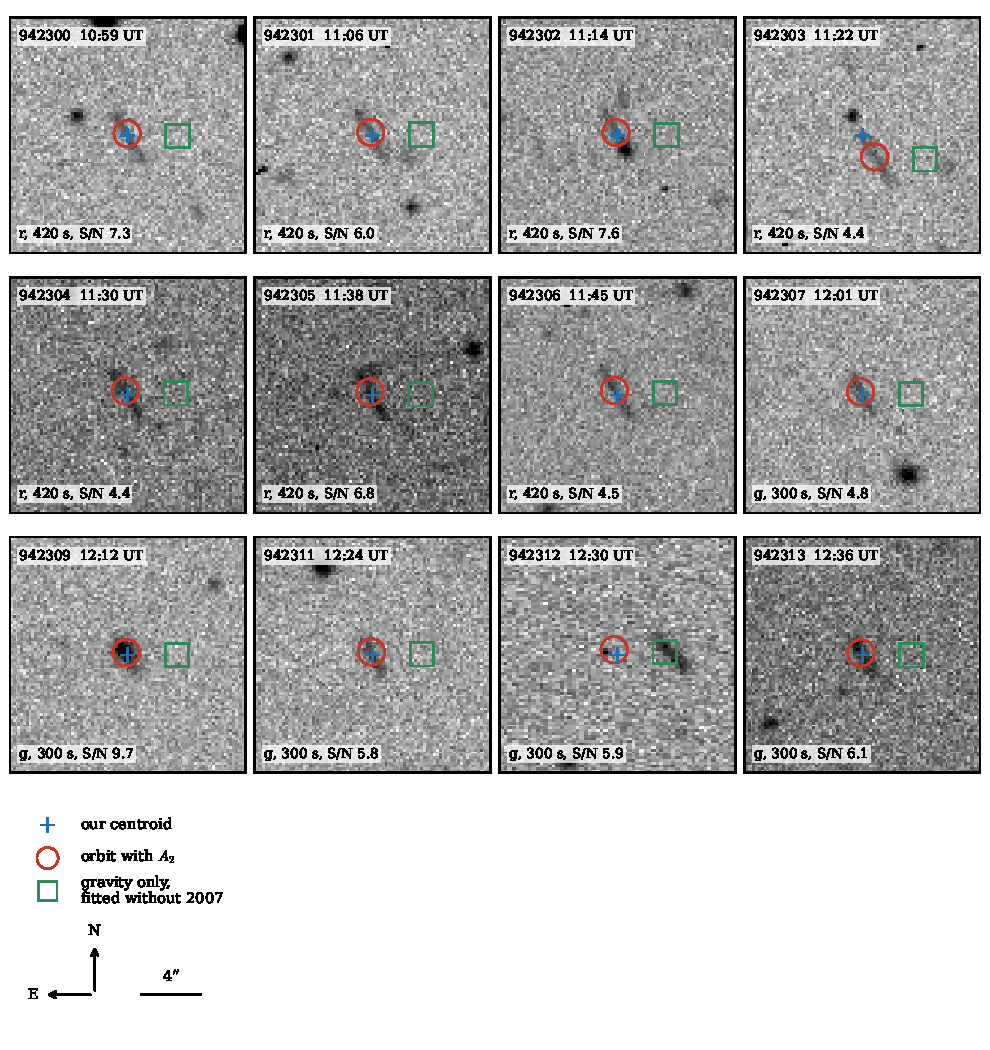
\includegraphics[width=0.92\textwidth]{cfht2007_cutouts.pdf}
\caption{2016 TA56 in the twelve CFHT MegaCam frames of 2007 September 14 in which it is
detected, $16''$ across, north up and east left: our centroid (cross), the position
predicted by the orbit with $A_2$ (circle) and the position predicted by the gravity-only
orbit fitted to the later apparitions (square). The object is trailed toward the
southwest by its motion during each exposure.}
\label{fig:cutouts}
\end{figure}

\begin{figure}[tbp]
\centering
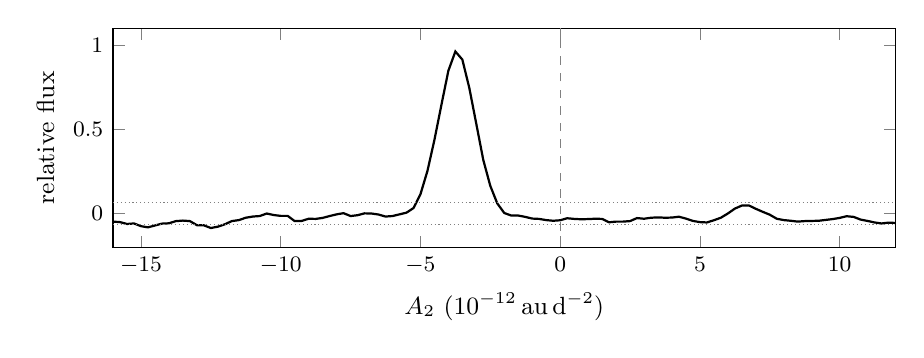
\begin{tikzpicture}
\begin{axis}[width=0.95\textwidth,height=0.36\textwidth,xmin=-16,xmax=12,ymin=-0.2,ymax=1.1,xlabel={$A_2$ ($10^{-12}$\,au\,d$^{-2}$)},ylabel={relative flux},tick label style={font=\footnotesize},label style={font=\small}]
\addplot[black,thick] coordinates {(-16.00,-0.047) (-15.75,-0.050) (-15.50,-0.061) (-15.25,-0.058) (-15.00,-0.074) (-14.75,-0.081) (-14.50,-0.070) (-14.25,-0.059) (-14.00,-0.057) (-13.75,-0.044) (-13.50,-0.041) (-13.25,-0.044) (-13.00,-0.068) (-12.75,-0.069) (-12.50,-0.085) (-12.25,-0.077) (-12.00,-0.063) (-11.75,-0.044) (-11.50,-0.038) (-11.25,-0.024) (-11.00,-0.017) (-10.75,-0.014) (-10.50,0.001) (-10.25,-0.008) (-10.00,-0.013) (-9.75,-0.013) (-9.50,-0.044) (-9.25,-0.043) (-9.00,-0.030) (-8.75,-0.031) (-8.50,-0.025) (-8.25,-0.014) (-8.00,-0.004) (-7.75,0.003) (-7.50,-0.014) (-7.25,-0.009) (-7.00,0.002) (-6.75,0.001) (-6.50,-0.005) (-6.25,-0.017) (-6.00,-0.014) (-5.75,-0.004) (-5.50,0.006) (-5.25,0.033) (-5.00,0.115) (-4.75,0.253) (-4.50,0.437) (-4.25,0.645) (-4.00,0.848) (-3.75,0.962) (-3.50,0.914) (-3.25,0.745) (-3.00,0.532) (-2.75,0.318) (-2.50,0.165) (-2.25,0.061) (-2.00,0.004) (-1.75,-0.011) (-1.50,-0.011) (-1.25,-0.019) (-1.00,-0.029) (-0.75,-0.031) (-0.50,-0.038) (-0.25,-0.042) (0.00,-0.039) (0.25,-0.027) (0.50,-0.031) (0.75,-0.033) (1.00,-0.032) (1.25,-0.030) (1.50,-0.031) (1.75,-0.051) (2.00,-0.047) (2.25,-0.047) (2.50,-0.044) (2.75,-0.026) (3.00,-0.030) (3.25,-0.024) (3.50,-0.022) (3.75,-0.024) (4.00,-0.023) (4.25,-0.018) (4.50,-0.029) (4.75,-0.043) (5.00,-0.050) (5.25,-0.052) (5.50,-0.039) (5.75,-0.024) (6.00,0.001) (6.25,0.030) (6.50,0.048) (6.75,0.049) (7.00,0.029) (7.25,0.011) (7.50,-0.006) (7.75,-0.030) (8.00,-0.038) (8.25,-0.042) (8.50,-0.047) (8.75,-0.044) (9.00,-0.043) (9.25,-0.042) (9.50,-0.037) (9.75,-0.032) (10.00,-0.025) (10.25,-0.015) (10.50,-0.019) (10.75,-0.035) (11.00,-0.043) (11.25,-0.052) (11.50,-0.058) (11.75,-0.053) (12.00,-0.055)};
\addplot[black!50,densely dotted] coordinates {(-16,0.066) (12,0.066)};
\addplot[black!50,densely dotted] coordinates {(-16,-0.066) (12,-0.066)};
\addplot[black!50,dashed] coordinates {(0,-0.2) (0,1.1)};
\end{axis}
\end{tikzpicture}
\caption{Median flux over the 2007 frames that measure each position, in units of the
detection's, of a source moving with 2016 TA56 at each position that orbits fitted to the
later apparitions allow,
labelled by the value of $A_2$ that places the object there. The dashed line marks the
gravity-only orbit ($A_2=0$) and the dotted lines $\pm3$ times the scatter at a fixed point
along lines displaced across the field.}
\label{fig:locus}
\end{figure}

\subsection{Size, albedo and the radiation bound}

NEOWISE detected 2016 TA56 twenty times: eight times in 2016 December at $1.61$ to
$1.62$\,au from the Sun and twelve times in 2017 June at $1.39$ to $1.40$\,au, at phase
angles of $37$ to $47^\circ$. Sixteen W2 fluxes reach S/N $4$ after the rejection of one
that differs by a magnitude from the rest of its apparition. At $\eta=1.4$ the fit gives
$D=2.44\pm0.06$\,km and $p_V=0.017$, with $\chi^2=28.4$ for $16$ fluxes, an uncertainty
conditional on that value of $\eta$; $\eta$ from $0.9$ to $1.9$ gives $D=1.41$ to
$3.72$\,km and $p_V=0.050$ to $0.007$ with nearly equal $\chi^2$, because W2 alone does not
constrain $\eta$ (Table~\ref{tab:thermal}), and this range is the uncertainty of the
diameter. Of the other assumptions, an emissivity of
$0.95$ increases $D$ by $5$ per cent, while the phase slope ($G=0.05$ or $0.25$), the ratio
of infrared to visible albedo ($1.0$ or $2.0$) and the flux floor ($5$ or $20$ per cent)
change it by less than $1$ per cent. The ten W1 measurements that reach S/N $4$ lie $0.6$
to $4.5$\,mag above the model and scatter by two magnitudes within an apparition, and one
of them coincides with a W2 measurement at S/N $2$, as expected for faint single-exposure
detections and blends with stars; they are not used. Table~S2 of the supplementary
material lists all twenty detections with their W1 and W2 magnitudes, uncertainties and
quality flags, and the use made of each. The JPL database,
which includes the NEOWISE diameters from the Planetary Data System, gives none for
2016 TA56; for the dark comet 2005 UY6, which has the same $H$, it gives $2.25$\,km and an
albedo of $0.018$ \citep{Masiero2017}, and for 2012 UR158 $0.63$\,km and $0.023$. Albedos
near $0.02$ are typical of cometary nuclei.

\begin{table}[t]
\centering\small
\caption{NEATM fits to the $16$ W2 fluxes of 2016 TA56 at fixed beaming parameters, with
the efficiency $\xi$ of the refitted $A_2$ relative to the radiation limit at
$1000$\,kg\,m$^{-3}$.}
\label{tab:thermal}
\begin{adjustbox}{max width=\textwidth}
\begin{tabular}{rrrrr}
\toprule
$\eta$ & $D$ (km) & $p_V$ & $\chi^2$ & $\xi$ \\
\midrule
0.9 & 1.41 & 0.050 & 31.0 & 14.7 \\
1.0 & 1.60 & 0.039 & 30.2 & 16.7 \\
1.2 & 2.00 & 0.025 & 29.1 & 20.8 \\
1.4 & 2.44 & 0.017 & 28.4 & 25.4 \\
1.6 & 2.92 & 0.012 & 28.0 & 30.4 \\
1.9 & 3.72 & 0.007 & 27.8 & 38.7 \\
\bottomrule
\end{tabular}
\end{adjustbox}
\end{table}

At the fitted diameter the refitted acceleration is $\xi=12.7$, $25.4$ and $50.8$ times
the radiation limit at $500$, $1000$ and $2000$\,kg\,m$^{-3}$; across the range of $\eta$
it is $7$ to $19$ times the limit at $500$\,kg\,m$^{-3}$. No bulk density between $500$
and $2000$\,kg\,m$^{-3}$ brings the acceleration within the radiation limit for any
beaming parameter from $0.9$ to $1.9$.

\subsection{Minimum outgassing rate}

Gas leaving the surface at about $0.5$\,km\,s$^{-1}$ imparts the largest transverse
momentum when all of it is emitted along track, so the acceleration sets a lower limit on
the production rate, $\dot M \ge M A_2\,g(r)/v$. At $D=2.44$\,km and $1000$\,kg\,m$^{-3}$
the mass is $7.6\times10^{12}$\,kg and the limit is $1.1$\,kg\,s$^{-1}$ of water
($3.6\times10^{25}$\,molecules\,s$^{-1}$) at $1$\,au and $3.1$\,kg\,s$^{-1}$ at the
perihelion distance of $0.59$\,au; at $500$\,kg\,m$^{-3}$ it is half as large. Gas
leaving at an angle $\theta$ to the track supplies only $\cos\theta$ of its momentum along
it, and the required rate rises by $1/\cos\theta$. These are production rates of weakly
active comets. The acceleration sets a lower limit rather than
the actual rate, and no coma has been reported for 2016 TA56; the activity of 1998 SH2
was not visible in archival images and was detected only with large-aperture
imaging \citep{Farnocchia2026}.

\subsection{The 2030 apparition}

The accelerated orbit and the gravity-only orbit fitted without the precovery agree to
within $0.2''$ until 2026 August, when the object fades below $V=22.4$. At the next
apparition they diverge: by $6.7''$ on 2030 July 30 at $V=20.2$ and solar elongation
$60^\circ$, by $4.0''$ on 2030 September 8 at $V=21.2$, and by $2.1''$ on 2030 October 18
at $V=22.4$. Propagating the fit covariances, the predicted position of each orbit is
uncertain almost entirely along the direction of separation, by $1.18''$ for the orbit
with $A_2$ and $0.71''$ for the gravity-only orbit on July 30 with one position per night,
and by less than $0.1''$ across it (Table~\ref{tab:pred}). A single position accurate to
$0.2''$ at any time from July 30 to September 28 therefore distinguishes the two orbits at
$4.6$ to $4.7\sigma$ with one position per night and at $6.9$ to $7.5\sigma$ with site
weights. These significances assume that both orbits are correct up to their fit
covariances. The apparition also measures the acceleration without the precovery: added to
the 2016 to 2026 positions without the 2007 night, a single position accurate to $0.2''$
on 2030 July 30 gives $\sigma(A_2)=0.39\times10^{-12}$\,au\,d$^{-2}$ with one position per
night, against $6.8\times10^{-12}$ from those positions alone, and three or six positions
spread over the apparition give $0.38$ and $0.37\times10^{-12}$, the uncertainty of the
state then dominating. Observations in 2030 can therefore confirm or exclude a term of the
fitted size at about $9\sigma$ whether or not the 2007 source is 2016 TA56. Table~S3 of the
supplementary material gives daily positions of both orbits from 2030 June to November
with their $1\sigma$ ellipses. Deep imaging at the same apparition, with the object $1.0$
to $1.6$\,au from the Sun, could detect the coma implied by the acceleration, as
large-aperture imaging did for 1998 SH2 \citep{Farnocchia2026}.

\begin{table}[t]
\centering\small
\caption{The orbit with $A_2$ and the gravity-only orbit fitted without 2007 at the 2030
apparition, seen from the geocentre: their separation, the $1\sigma$ uncertainty of each
along the separation from its fit covariance, and the significance with which a single
position accurate to $0.2''$ distinguishes them, with one position per night and with
site weights.}
\label{tab:pred}
\begin{adjustbox}{max width=\textwidth}
\begin{tabular}{lrrrrrrrr}
\toprule
 & \multicolumn{4}{c}{One position a night} & \multicolumn{4}{c}{Site weights} \\
\cmidrule(lr){2-5}\cmidrule(lr){6-9}
Date & Sep.\ ($''$) & $\sigma_{A_2}$ ($''$) & $\sigma_{\rm grav}$ ($''$) & $\sigma$ & Sep.\ ($''$) & $\sigma_{A_2}$ ($''$) & $\sigma_{\rm grav}$ ($''$) & $\sigma$ \\
\midrule
2030 July 30 & 6.55 & 1.18 & 0.71 & 4.7 & 6.72 & 0.72 & 0.49 & 7.5 \\
2030 August 19 & 5.36 & 0.95 & 0.58 & 4.7 & 5.49 & 0.59 & 0.40 & 7.5 \\
2030 September 8 & 3.89 & 0.68 & 0.42 & 4.7 & 4.00 & 0.42 & 0.29 & 7.3 \\
2030 September 28 & 2.76 & 0.48 & 0.30 & 4.6 & 2.84 & 0.29 & 0.20 & 6.9 \\
\bottomrule
\end{tabular}
\end{adjustbox}
\end{table}

\subsection{Overview of the tests}\label{sec:summary}

Table~\ref{tab:tests} lists the main tests of the acceleration of 2016 TA56 and the
alternative explanation each addresses. The first six measure the significance of the term
and whether measurement errors could produce it, all on the assumption that the 2007
source is 2016 TA56; the significance of the fit does not test that assumption. The search
of the allowed positions and the census of moving sources test the identification itself,
in the 2007 images. The radiation limit concerns the cause of the measured term, and the
2030 apparition will test the result independently of the precovery.

\begin{table}[tbp]
\centering\small\linespread{1.0}\selectfont
\caption{Tests of the transverse acceleration of 2016 TA56, the alternative each addresses
and its result.}
\label{tab:tests}
\begin{adjustbox}{max width=\textwidth}
\begin{tabular}{>{\raggedright\arraybackslash}p{0.27\textwidth}>{\raggedright\arraybackslash}p{0.29\textwidth}>{\raggedright\arraybackslash}p{0.36\textwidth}}
\toprule
Test & Alternative addressed & Result \\
\midrule
Fit of all $102$ positions & A statistical fluctuation & $9\sigma$ with each night as one
position, $13\sigma$ under the night-level covariance, $6.5\sigma$ from the night jackknife \\
Error shared by the 2007 positions & Correlated errors within the precovery night & $1.2''$
needed to bring $A_2$ below $3\sigma$ \\
2007 offset across the motion & A clock error in the precovery reports & $3.0''$ across
the motion, $15$ times the prediction uncertainty \\
Independent measurement of the CFHT frames & An error in either report's reduction or catalogue &
The offset is in the images; both reports lie $0.10''$ rms from our track \\
Radial term fitted with $A_2$ & A radial force mimicking a transverse one & $A_1$
at $2\sigma$; $A_2$ unchanged \\
Gravity-only orbit through 2007 to 2022 & A gravity-only orbit that fits the precovery &
It misses the 2025 positions by $10.5''$ \\
Positions allowed by the later apparitions & The precovery is another object & One source
among them; nothing at the gravity-only position to $3.9$\,mag below it \\
Census of moving sources in the 2007 frames & An unrelated object moving as predicted &
None within $5''$ per hour and $10^\circ$ of the motion; $8\times10^{-6}$ expected within
$30''$ \\
NEOWISE diameter and the radiation limit & Thermal recoil or radiation pressure & $15$ to
$39$ times the limit; significant drifts have a median of $0.075$ of it \\
The 2030 apparition & All of the above & One position gives
$\sigma(A_2)=0.39\times10^{-12}$\,au\,d$^{-2}$ without the precovery \\
\bottomrule
\end{tabular}
\end{adjustbox}
\end{table}

\subsection{1998 SH2 and 2006 VC}\label{sec:others}

Applying the same fits and thermal model to the two further objects identified by the
screen at $2000$\,kg\,m$^{-3}$ and albedo $0.14$ (Table~\ref{tab:others}) confirms an
acceleration for one of them but not for the other.

(875163) 1998 SH2 ($a=2.74$\,au, $e=0.71$, $q=0.79$\,au, $i=2.4^\circ$, $T_J=2.91$) has
$404$ positions in three apparitions: $48$ at its discovery in 1998 September, $104$ from
2016 February to October and $252$ from 2025 August to October. With site weights, the fit
with $A_2$ retains $379$ positions at an rms of $0.30''$ and gives
$A_2=(-6.11\pm0.24)\times10^{-13}$\,au\,d$^{-2}$; with one position per night it gives
$(-6.45\pm0.54)\times10^{-13}$, a $12\sigma$ detection, and with a radial term ($0.4\sigma$)
included it gives $(-6.18\pm0.30)\times10^{-13}$, compared with JPL's
$(-6.96\pm0.49)\times10^{-13}$. The gravity-only fit retains $354$ positions at
$\chi^2$/dof $0.90$, against $0.67$ with $A_2$. As for 2016 TA56, the earliest apparition
deviates most from a gravity-only orbit: the gravity-only orbit fitted to 2016 and 2025,
which predicts the 1998 September positions to $0.52''$ along and $0.21''$ across the
apparent motion, is offset from the discovery positions by $13.0''$ along and $5.3''$
across the motion, and a timing error cannot produce the cross-track offset. Fits omitting
one apparition give $A_2=-4.3\pm1.2$, $-1.8\pm0.6$ and
$-1.9\pm2.1\times10^{-12}$\,au\,d$^{-2}$, all of the same sign but two of them $2$ to
$3\sigma$ larger than the full-arc value, so the magnitude of the term is less certain
than its formal uncertainty. NEOWISE detected the object six times in W2 at $1.14$\,au
from the Sun and phase angles of $58$ to $59^\circ$: at $\eta=1.4$ the fit gives
$D=0.64$\,km and $p_V=0.019$, and $\eta$ from $0.9$ to $1.9$ gives $0.39$ to $0.93$\,km
and $0.051$ to $0.009$; the NEOWISE catalogue gives $0.38\pm0.06$\,km and
$0.058\pm0.024$ \citep{Masiero2017}, matching our fit at $\eta=0.9$. The acceleration is
then $0.7$ to $1.7$ times the radiation limit at $1000$\,kg\,m$^{-3}$ across this range,
and $0.7$ times at the catalogue diameter. It lies within the limit for the smaller sizes,
but only if more than half of the re-emitted momentum were directed along track, whereas
the thermal lag of the Yarkovsky effect directs at most about a
tenth \citep{Vokrouhlicky2015}. A dark body of $0.4$ to $0.9$\,km on a Jupiter-family
orbit, with an acceleration that radiation forces cannot plausibly produce, matches the
outer dark comets; at the catalogue diameter and $1000$\,kg\,m$^{-3}$ the minimum
outgassing rate is $8\times10^{-4}$\,kg\,s$^{-1}$ of water at $1$\,au. \citet{Farnocchia2026} showed that it is a comet: they found these perturbations in
its 1998--2025 astrometry and, in large-aperture images taken during its 2025 August
close approach, a weak tail of low surface brightness not seen in archival images. The
screen, with the generic thresholds of Section~\ref{sec:method}, and the orbit analysis
applied to 2016 TA56 therefore recover an independently confirmed, weakly active comet
from its acceleration alone; relative to the radiation limit at the same beaming
parameter, the acceleration of 2016 TA56 is twenty times larger. The recovery is
retrospective, since the activity of 1998 SH2 was reported before the screen was run, so
it shows that the screen is sensitive to weakly active comets but is not a blind
prediction, and it does not by itself establish that 2016 TA56 is one.

(428209) 2006 VC ($a=1.94$\,au, $e=0.49$, $q=0.99$\,au, $T_J=3.72$), not detected by
NEOWISE, has $216$ positions in four apparitions from 2006 to 2026. The fit with $A_2$
gives $(+5.5\pm0.9)\times10^{-13}$\,au\,d$^{-2}$, and $(+6.7\pm1.5)\times10^{-13}$ with one
position per night, but the gravity-only fit is equally good ($\chi^2$/dof $0.96$ against
$0.95$, with two fewer positions retained), and omitting the apparition of 2025 October to
2026 May gives $(+5.7\pm8.7)\times10^{-13}$. The term therefore comes from that apparition
alone, and the present arc does not require an acceleration. The two orbits diverge from
2033 September, by up to $25''$ in 2034 February at $V=19.8$.

\begin{table}[t]
\centering\small
\caption{Orbit fits of 1998 SH2 and 2006 VC to the MPC positions, as in
Table~\ref{tab:fits}.}
\label{tab:others}
\begin{adjustbox}{max width=\textwidth}
\begin{tabular}{llrrrl}
\toprule
Object & Fit & Positions & Kept & $\chi^2$/dof & $A_2$ ($10^{-13}$\,au\,d$^{-2}$) \\
\midrule
1998 SH2 & with $A_2$, site weights & 404 & 379 & 504.4/751 & $-6.11\pm0.24$ \\
 & with $A_2$, one position a night & 404 & 401 & 130.7/795 & $-6.45\pm0.54$ \\
 & with $A_1$ and $A_2$ & 404 & 379 & 504.3/750 & $-6.18\pm0.30$ \\
 & gravity only & 404 & 354 & 634.8/702 & --- \\
 & without 1998 September & 356 & 342 & 442.4/677 & $-42.7\pm12.3$ \\
 & without 2016 & 300 & 284 & 328.3/561 & $-18.0\pm5.7$ \\
 & without 2025 & 152 & 135 & 210.4/263 & $-19.0\pm21.1$ \\
2006 VC & with $A_2$, site weights & 216 & 185 & 345.0/363 & $+5.54\pm0.94$ \\
 & with $A_2$, one position a night & 216 & 213 & 143.2/419 & $+6.66\pm1.47$ \\
 & gravity only & 216 & 183 & 343.9/360 & --- \\
 & without 2025--2026 & 193 & 163 & 316.6/319 & $+5.65\pm8.65$ \\
\bottomrule
\end{tabular}
\end{adjustbox}
\end{table}

% =============================================================================
\section{Relation to previous work}\label{sec:related}
% =============================================================================

\citet{Farnocchia2013} established the systematic detection of
Yarkovsky drifts in near-Earth asteroid astrometry and the comparison of these drifts with
the radiation force. \citet{Seligman2023} identified the first dark comets
among bodies whose accelerations exceed that force, and their later
sample \citep{Seligman2024} separated the inner and outer populations. \citet{Taylor2024a} traced the dynamical origins of the dark comets and proposed an
evolutionary track through rotational fragmentation, and \citet{Taylor2024b}
examined how strong non-gravitational accelerations affect the linking of observations.
\citet{Farnocchia2026} attributed the non-gravitational perturbations of
1998 SH2 to cometary activity by imaging its weak tail, suggested that more near-Earth
objects classified as asteroids could be comets with undetected outgassing, and called
for systematic searches; the screen presented here is such a search over every
transverse term in JPL's database. We are not aware of any earlier report of a
non-gravitational acceleration of 2016 TA56 beyond JPL's orbit solution.

% =============================================================================
\section{Conclusion}\label{sec:conclusion}
% =============================================================================

Among the transverse accelerations in JPL's database, that of 2016 TA56 exceeds the
radiation limit by a factor that no plausible density or albedo removes, while the
significant drifts of the database have a median efficiency of $0.075$. The object is on a
Jupiter-family orbit like those of the outer dark comets and has not previously been
listed among them. Its acceleration is measured conditionally on the 2007 precovery. With
that night the fit gives $9\sigma$ when each night counts as one position and $13\sigma$
under a night-level covariance estimated from the residuals; the uncertainty from refits
that each omit one later night corresponds to $6.5\sigma$; and the twelve precovery
positions would have to share an error of $1.2''$ to bring the term below $3\sigma$.
Without that night the later apparitions do not measure it. The 2007 images identify the
precovery source with 2016 TA56: among all positions that orbits fitted to the later
apparitions allow, it is the only source, nothing lies at the gravity-only position to
$3.9$\,mag below it, and no other moving source in the frames shares its motion. NEOWISE
indicates a dark body about $2.4$\,km across, similar to the dark comet 2005 UY6. All
drifts with known spin poles have the sign expected from the spin. The same screen and
orbit analysis recover, retrospectively, the weakly active comet 1998 SH2 from an
acceleration $0.7$ to $1.7$ times the radiation limit at $1000$\,kg\,m$^{-3}$; over the
same range of beaming parameters the acceleration of 2016 TA56 is $15$ to $39$ times the
limit. The orbit fit measures a transverse term and the thermal fit shows that radiation
forces cannot produce it, but no coma has been reported, and outgassing is an inference
from the size of the term; 2016 TA56 is a candidate dark comet, not a confirmed comet. The
2030 apparition tests the result independently of the precovery: the two orbits then
diverge by $4$ to $7''$ at $V\approx20$ to $21$, a single position accurate to $0.2''$
would measure $A_2$ to $\pm0.4\times10^{-12}$\,au\,d$^{-2}$ without the 2007 night, and
deep imaging could detect the faint coma that outgassing at this rate implies. For the
third object, 2006 VC, the term depends on its latest apparition alone. The screen covers
only the $611$ asteroids for which JPL has fitted a transverse term, $609$ of the
$42{,}772$ known near-Earth asteroids among them; it finds candidates among measured
accelerations and does not measure the abundance of dark comets.

\section*{Acknowledgements}

This work uses observations from the Minor Planet Center; orbit solutions and ephemerides
from JPL's Solar System Dynamics group through the Small-Body Database and Horizons; the
NEOWISE single-exposure source table from the NASA/IPAC Infrared Science Archive; the
DAMIT database; and the software ASSIST, REBOUND, astropy, NumPy and SciPy.

\section*{Data availability}

The analysis software and the derived results are available at
\begin{center}
\href{https://github.com/CharlesCNorton/seti-tools/tree/main/papers/dark_comet}{\nolinkurl{https://github.com/CharlesCNorton/seti-tools}}
\end{center}
\noindent in the directory \texttt{papers/dark\_comet}, where a README lists each data file
behind the tables and figures and the command that produces it. Tables S1 to S3 are in the supplementary material. The observations,
orbit solutions, NEOWISE detections, CFHT images and spin models are publicly available
from the archives cited in the text.

\begin{thebibliography}{99}
\expandafter\ifx\csname natexlab\endcsname\relax\def\natexlab#1{#1}\fi

\bibitem[{Astropy Collaboration et~al.(2022)}]{Astropy2022}
Astropy Collaboration, Price-Whelan, A.M., Lim, P.L., et al., 2022. The Astropy Project:
sustaining and growing a community-oriented open-source project and the latest major release
(v5.0) of the core package. Astrophys. J. 935, 167. \href{https://doi.org/10.3847/1538-4357/ac7c74}{doi:\nolinkurl{10.3847/1538-4357/ac7c74}}

\bibitem[{Berthier et~al.(2006)}]{Berthier2006}
Berthier, J., Vachier, F., Thuillot, W., et al., 2006. SkyBoT, a new VO service to identify
Solar System objects. In: Gabriel, C., Arviset, C., Ponz, D., Solano, E. (Eds.), Astronomical
Data Analysis Software and Systems XV. ASP Conf. Ser. 351, 367.

\bibitem[{Bowell et~al.(1989)}]{Bowell1989}
Bowell, E., Hapke, B., Domingue, D., Lumme, K., Peltoniemi, J., Harris, A.W., 1989.
Application of photometric models to asteroids. In: Binzel, R.P., Gehrels, T., Matthews,
M.S. (Eds.), Asteroids II. Univ. of Arizona Press, Tucson, pp. 524--556.

\bibitem[{{\v{D}}urech et~al.(2010)}]{Durech2010}
{\v{D}}urech, J., Sidorin, V., Kaasalainen, M., 2010. DAMIT: a database of asteroid models.
Astron. Astrophys. 513, A46. \href{https://doi.org/10.1051/0004-6361/200912693}{doi:\nolinkurl{10.1051/0004-6361/200912693}}

\bibitem[{Farnocchia et~al.(2013)}]{Farnocchia2013}
Farnocchia, D., Chesley, S.R., Vokrouhlick{\'y}, D., Milani, A., Spoto, F., Bottke, W.F.,
2013. Near Earth Asteroids with measurable Yarkovsky effect. Icarus 224, 1--13.
\href{https://doi.org/10.1016/j.icarus.2013.02.004}{doi:\nolinkurl{10.1016/j.icarus.2013.02.004}}

\bibitem[{Farnocchia et~al.(2026)}]{Farnocchia2026}
Farnocchia, D., Hainaut, O.R., Seligman, D.Z., et al., 2026. Non-gravitational acceleration
indicative of cometary activity of near-Earth object. Nat. Astron. 10, 1283--1291.
\href{https://doi.org/10.1038/s41550-026-02913-7}{doi:\nolinkurl{10.1038/s41550-026-02913-7}}

\bibitem[{Harris(1998)}]{Harris1998}
Harris, A.W., 1998. A thermal model for near-Earth asteroids. Icarus 131, 291--301.
\href{https://doi.org/10.1006/icar.1997.5865}{doi:\nolinkurl{10.1006/icar.1997.5865}}

\bibitem[{Holman et~al.(2023)}]{Holman2023}
Holman, M.J., Akmal, A., Farnocchia, D., et al., 2023. ASSIST: an ephemeris-quality
test-particle integrator. Planet. Sci. J. 4, 69. \href{https://doi.org/10.3847/PSJ/acc9a9}{doi:\nolinkurl{10.3847/PSJ/acc9a9}}

\bibitem[{Mainzer et~al.(2011)}]{Mainzer2011}
Mainzer, A., Grav, T., Masiero, J., et al., 2011. Thermal model calibration for minor planets
observed with Wide-field Infrared Survey Explorer/NEOWISE. Astrophys. J. 736, 100.
\href{https://doi.org/10.1088/0004-637X/736/2/100}{doi:\nolinkurl{10.1088/0004-637X/736/2/100}}

\bibitem[{Mainzer et~al.(2014)}]{Mainzer2014}
Mainzer, A., Bauer, J., Cutri, R.M., et al., 2014. Initial performance of the NEOWISE
reactivation mission. Astrophys. J. 792, 30. \href{https://doi.org/10.1088/0004-637X/792/1/30}{doi:\nolinkurl{10.1088/0004-637X/792/1/30}}

\bibitem[{Marsden et~al.(1973)}]{Marsden1973}
Marsden, B.G., Sekanina, Z., Yeomans, D.K., 1973. Comets and nongravitational forces. V.
Astron. J. 78, 211. \href{https://doi.org/10.1086/111402}{doi:\nolinkurl{10.1086/111402}}

\bibitem[{Masiero et~al.(2017)}]{Masiero2017}
Masiero, J.R., Nugent, C., Mainzer, A.K., et al., 2017. NEOWISE reactivation mission year
three: asteroid diameters and albedos. Astron. J. 154, 168.
\href{https://doi.org/10.3847/1538-3881/aa89ec}{doi:\nolinkurl{10.3847/1538-3881/aa89ec}}

\bibitem[{Park et~al.(2021)}]{Park2021}
Park, R.S., Folkner, W.M., Williams, J.G., Boggs, D.H., 2021. The JPL planetary and lunar
ephemerides DE440 and DE441. Astron. J. 161, 105. \href{https://doi.org/10.3847/1538-3881/abd414}{doi:\nolinkurl{10.3847/1538-3881/abd414}}

\bibitem[{Rein and Liu(2012)}]{Rein2012}
Rein, H., Liu, S.-F., 2012. REBOUND: an open-source multi-purpose N-body code for
collisional dynamics. Astron. Astrophys. 537, A128. \href{https://doi.org/10.1051/0004-6361/201118085}{doi:\nolinkurl{10.1051/0004-6361/201118085}}

\bibitem[{Rein and Spiegel(2015)}]{Rein2015}
Rein, H., Spiegel, D.S., 2015. IAS15: a fast, adaptive, high-order integrator for
gravitational dynamics, accurate to machine precision over a billion orbits. Mon. Not. R.
Astron. Soc. 446, 1424--1437. \href{https://doi.org/10.1093/mnras/stu2164}{doi:\nolinkurl{10.1093/mnras/stu2164}}

\bibitem[{Seligman et~al.(2023)}]{Seligman2023}
Seligman, D.Z., Farnocchia, D., Micheli, M., et al., 2023. Dark comets? Unexpectedly large
nongravitational accelerations on a sample of small asteroids. Planet. Sci. J. 4, 35.
\href{https://doi.org/10.3847/PSJ/acb697}{doi:\nolinkurl{10.3847/PSJ/acb697}}

\bibitem[{Seligman et~al.(2024)}]{Seligman2024}
Seligman, D.Z., Farnocchia, D., Micheli, M., et al., 2024. Two distinct populations of dark
comets delineated by orbits and sizes. Proc. Natl. Acad. Sci. U.S.A. 121, e2406424121.
\href{https://doi.org/10.1073/pnas.2406424121}{doi:\nolinkurl{10.1073/pnas.2406424121}}

\bibitem[{Taylor et~al.(2024{\natexlab{a}})}]{Taylor2024a}
Taylor, A.G., Steckloff, J.K., Seligman, D.Z., et al., 2024a. The dynamical origins of the dark
comets and a proposed evolutionary track. Icarus 420, 116207.
\href{https://doi.org/10.1016/j.icarus.2024.116207}{doi:\nolinkurl{10.1016/j.icarus.2024.116207}}

\bibitem[{Taylor et~al.(2024{\natexlab{b}})}]{Taylor2024b}
Taylor, A.G., Seligman, D.Z., Holman, M.J., et al., 2024b. Strong nongravitational
accelerations and the potential for misidentification of near-Earth objects. Astrophys. J.
976, 190. \href{https://doi.org/10.3847/1538-4357/ad85e3}{doi:\nolinkurl{10.3847/1538-4357/ad85e3}}

\bibitem[{Vere{\v{s}} et~al.(2017)}]{Veres2017}
Vere{\v{s}}, P., Farnocchia, D., Chesley, S.R., Chamberlin, A.B., 2017. Statistical analysis
of astrometric errors for the most productive asteroid surveys. Icarus 296, 139--149.
\href{https://doi.org/10.1016/j.icarus.2017.05.021}{doi:\nolinkurl{10.1016/j.icarus.2017.05.021}}

\bibitem[{Vokrouhlick{\'y} et~al.(2015)}]{Vokrouhlicky2015}
Vokrouhlick{\'y}, D., Bottke, W.F., Chesley, S.R., Scheeres, D.J., Statler, T.S., 2015. The
Yarkovsky and YORP effects. In: Michel, P., DeMeo, F.E., Bottke, W.F. (Eds.), Asteroids IV.
Univ. of Arizona Press, Tucson, pp. 509--531.
\href{https://doi.org/10.2458/azu_uapress_9780816532131-ch027}{doi:\nolinkurl{10.2458/azu_uapress_9780816532131-ch027}}

\bibitem[{Wright et~al.(2010)}]{Wright2010}
Wright, E.L., Eisenhardt, P.R.M., Mainzer, A.K., et al., 2010. The Wide-field Infrared Survey
Explorer (WISE): mission description and initial on-orbit performance. Astron. J. 140,
1868--1881. \href{https://doi.org/10.1088/0004-6256/140/6/1868}{doi:\nolinkurl{10.1088/0004-6256/140/6/1868}}

\end{thebibliography}

\end{document}
